%%%%%%%%%%%%%%%%%%%%%%
\chapter{Introduction}
%%%%%%%%%%%%%%%%%%%%%%

% \todo{
% The introduction is a longer writeup that gently eases the reader into your
% thesis. Use the first paragraph to discuss the setting.
% In the second paragraph you can introduce the main challenge that you see.
% The third paragraph lists why related work is insufficient.
% The fourth and fifth paragraphs discuss your approach and why it is needed.
% The sixth paragraph will introduce your thesis statement. Think how you can
% distill the essence of your thesis into a single sentence.
% The seventh paragraph will highlight some of your results
% The eights paragraph discusses your core contribution.
% This section is usually 3-5 pages.}

\section{Decision-Focused Learning for ND Problems}

In operations research, we are often tasked with finding high-quality solutions to problems where not all the information is known at the time of planning. For instance, in the field of freight railroad scheduling, planners design a schedule that fulfills the demand for cargo between different origins and destinations. We use algorithms and methods from mathematical optimization to find the most appropriate schedule. However, railroad schedules are planned months in advance, well before the exact demand is known. We thus have to make predictions about demand ahead of time, using statistical methods.

In order to make high-quality decisions, operations researchers typically model the situation as a mathematical optimization problem, which aims to find solutions that minimize or maximize a cost function, while respecting a set of constraints. Commonly, such optimization problems can be written as Mixed-Integer Linear Programs (MILP). In the case of deterministic MILP problems, the cost function and the constraints are linear and their coefficients are fixed and known. The coefficients are also called the parameters of the model.

Optimization models are used to make long-term strategic decisions, sometimes months or years in advance, which means some model parameters are not known exactly at the time of planning and need to be predicted. Researchers use statistical prediction models, such as time series or Machine Learning (ML) models, that use contextual data to estimate the future value of the parameters. The process of using contextual data to predict parameters to an optimization model, then using that model to find high-quality decisions is called the data-decisions pipeline, illustrated in Figure \ref{fig:intro:data-decisions}.

\begin{figure}[ht]
    \centering
    \begin{tikzpicture}[main/.style={draw, rectangle, thick, minimum height=4cm, minimum width=3cm}]
\node[main] (pred) {\shortstack{\Large Predict\\\\
    \color{gray} \small e.g.\\
    \color{gray} \small Machine learning\\
    \color{gray} \small Time series
}};
\node[main] (opt) [right=of pred] {\shortstack{\Large            Optimize\\\\
    \color{gray} \small e.g.\\
    \color{gray} \small Operations\\
    \color{gray} \small research\\
    \color{gray}\small MILP
}};
\node (decision) [right=of opt] {};
\node (data) [left=of pred] {};

\draw[->,  thick] (pred.east) +(0, 0.1) to [out=45,in=135,looseness=1.3] (opt.west); 
\draw[->, thick] (opt.west) +(0, -0.1) to [out=-135,in=-45,looseness=1.3] (pred.east);    
\draw[->, thick] (data) -- node[near start, above] {Data} (pred); 
\draw[->, thick] (opt) -- node[near start, above, pos=0.9] {Decisions} (decision); 
\end{tikzpicture}

    \caption{The data-decisions pipeline}
    \label{fig:intro:data-decisions}
\end{figure}

This project focuses on predicting the demand coefficients in Network Design (ND) problems formulated as MILPs, which are particularly difficult to solve optimally.  From railroad scheduling to city logistics to airport hub placement, many problems in transportation and logistics can be formulated as ND problems. ND problems are defined on a graph consisting of nodes and arcs connecting them. Given a set of commodities: each commodity is transported from its origin node to its destination node according to its demand. The objective is to find the cheapest subset of arcs that satisfies the demand for every commodity while respecting the capacity of the arcs. This is a difficult problem to solve even if we assume that all model parameters are known in advance. In fact, not only is this problem computationally $\mathcal{NP}$-hard, but real-world instances are large, with tens of thousands of parameters, and standard approaches for approximating MILP solutions, such as Linear Program (LP) relaxations, work poorly on ND problems. 

The parameters of the ND model, such as arc capacity, design and flow costs, and commodity demands, are not known at the time of planning. Their values are uncertain and are predicted using statistical models. There are several ways to handle the uncertainty in the parameters. Stochastic Network Design \citep{alonso-ayusoApproachStrategicSupply2003} minimizes the expected costs over the probability distribution of the parameters. These models are computationally very difficult to optimize, and the parameter distributions are often hard to approximate. Robust Network Design \citep{kosterRobustNetworkDesign2013} considers that parameters occur within an uncertainty set, and minimizes the worst-case cost within that uncertainty set. Robust optimization is an emerging field: there is little research applied to ND problems, and it presents similar computational difficulties to Stochastic Network Design. Finally, the most common way to handle the uncertainty is to make point predictions for the ND parameters, and then solve the deterministic formulation of the ND problem. This has the advantage of being much easier to solve computationally, at the cost of losing the information about the parameter distribution in the optimization phase. The deterministic ND formulation is the one most commonly used in practice, but it requires special attention to make good point predictions.

In this work, we focus on making point predictions for commodity demands. This is because, in practice, demand has the highest uncertainty and is the most difficult to predict from historical data, compared to the other model parameters. In fact, even with a good estimation of the probability distribution, it is difficult to make good point predictions of demand. Furthermore, the demand parameters appear in the constraints of the ND model, which means that the predictions affect the feasible region of the optimization problem. Demand predictions will strongly affect the final network quality.  

We train statistical models to make demand predictions from contextual data. This is typically done separately from the solving the optimization problem, which can lead to a mismatch between prediction accuracy and downstream optimization cost. The prediction model is trained on a dataset of demands and associated contextual features. Given the contextual features, it produces a conditional point estimate of the demand. During training, the model iteratively minimizes a loss function that compares the predicted demand to the actual demand, such as Mean Squared Error (MSE) or Mean Absolute Error (MAE). These measures of accuracy do not take into account the effect of the prediction error on the optimization step. Over- or underpredicting demand can radically affect the cost of the resulting network, even if two predictions have the same loss function value. Thus, integrating the prediction and optimization steps by evaluating demand predictions on the cost of the downstream optimization problem, rather than on pure prediction accuracy, could result in better performing networks.

\section{An Illustrative Example of the Utility of Decision-Focused Learning}

To illustrate the utility of integrating the prediction and optimization steps of a data-decisions pipeline, consider the following example, shown in Figure \ref{fig:intro:example-network}. Suppose we are trying to build the lowest cost network for transporting a single commodity from its origin $s$ to its destination $t$. We have a choice of two possible arcs: the upper arc $p$ has a cheaper design cost $f_p = 10$ but has a limited capacity of $u_p = 16$, and the lower arc $q$ has a more expensive design cost of $f_q = 100$ but has unlimited capacity $u_q = \infty$. 

\begin{figure}[ht]
    \centering
     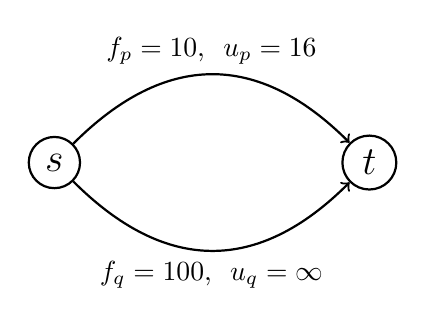
\begin{tikzpicture}[node distance={40mm}, thick, main/.style = {draw, circle}]
    \node[main] (s) {\Large $s$}; 
    \node[main] (t) [right of=s] {\Large $t$};
    \draw[->] (s) to [out=45, in=135, looseness=1.2] node[midway, above] { \green{$f_p = 10$}, \red{ $u_p = 16$}} (t); 
    \draw[->] (s) to [out=-45, in=-135, looseness=1.2] node[midway, below] {\green{$f_q = 100$}, \red{ $u_q = \infty$}} (t); 
\end{tikzpicture} 

    \caption{Example of a  single commodity network with two arcs: a cheap but limited capacity arc $p$, and an expensive but unlimited capacity arc $q$}
    \label{fig:intro:example-network}
\end{figure}

We will go into further detail in Chapter \ref{sec:litrev:network-design}, but for now let us assume that we can formulate the network in Figure \ref{fig:intro:example-network} as a mathematical optimization problem which we write $\mathrm{MCFND}(d)$, where $d$ is the commodity demand. Further assume that there exists a procedure to solve $\mathrm{MCFND}(d)$ and obtain the optimal network that satisfies the demand $d$.

\begin{figure}[ht]
    \centering
    \begin{tikzpicture}[model/.style={rectangle, minimum width=15mm, minimum height=10mm, draw, thick},
                demand/.style={text=blue}]
    \node (context) {\shortstack{Features \\$\bm{\phi}$}};
    \node[model] (model1) [below left=of context] {$f_{\theta_1}$};
    \node[model] (model2) [below right=of context] {$f_{\theta_2}$};
    \node[] (mse1) [below=of model1] {$\mathcal{L}_{\text{MSE}}(\hat{\bm{d}}_1, \bm{d}) = 1$};
    \node[] (mse2) [below=of model2] {$\mathcal{L}_{\text{MSE}}(\hat{\bm{d}}_2, \bm{d}) = 1$};
    
    \draw[->] (context.south) +(-0.5, 0) -- (model1.north);
    \draw[->] (context.south) +(0.5, 0) -- (model2.north);
    
    \draw[->] (model1) -- node[demand] (demand1) [right] {$\hat{d}_1 = 15$} (mse1);
    \draw[->] (model2) -- node[demand] (demand2) [right] {$\hat{d}_2 = 17$} (mse2);
    \draw[<->, draw=ForestGreen, very thick] (mse1) -- node[midway, fill=white] {\color{ForestGreen} $\mathbf{=}$} (mse2);
\end{tikzpicture}

    \caption{Comparing the predicted demands of two prediction models $f_1$ and $f_2$.}
    \label{fig:intro:example-prediction}
\end{figure}

We let actual demand for the commodity be $d = 16$, but this demand is uncertain and is predicted from the associated contextual features $\phi$. Consider the case of two prediction models $f_1$ and $f_2$, which, given the same contextual features $\phi$, output two different predictions for the demand  $\hat{d}_1 = f_1(\phi) = 15$ and $\hat{d}_2 = f_2(\phi) = 17$. If we evaluate these predictions with respect to the actual demand using standard evaluation metrics from machine learning, these two predictions obtain the same score. Indeed, in this case, both models obtain a Mean Squared Error score of $\mathcal{L}_{\text{MSE}}(\hat{d}_1, d) = \mathcal{L}_{\text{MSE}}(\hat{d}_2, d) = 1$. The two predictions made by these models are equivalent when measured in the prediction step, but this does not necessarily mean that the two predictions result the same downstream optimization cost.

In this example, equal prediction loss does not mean equal downstream optimization cost. Suppose we use each predicted demand in the MCFND to determine which arcs to build. In this case, we get two optimal networks with radically different costs, as shown in Figure \ref{fig:intro:example-optimization}. In this case, prediction models that slightly underpredict demand would result in a cheaper downstream network compared to models that overpredict demand. This example highlights the importance of integrating the prediction and optimization steps: training and evaluating prediction models using techniques that do not take into account the structure of the downstream optimization problem can lead to suboptimal decisions.

\begin{figure}[ht]
    \begin{multicols}{2}
        \centering $\text{MCFND}(\hat{d}_1 = 15)$ \vspace{2mm}
    
        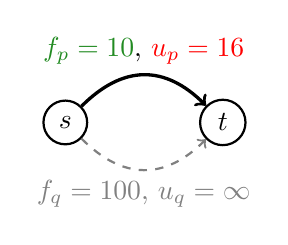
\begin{tikzpicture}[node distance={20mm}, thick, main/.style = {draw, circle}]
            \node[main] (s) {$s$}; 
            \node[main] (t) [right of=s] {$t$};
            \draw[->, very thick] (s) to [out=45, in=135, looseness=1.2] node[midway, above] { {\color{ForestGreen}$f_p = 10$}, {\color{Red} $u_p = 16$}} (t); 
            \draw[->, draw=gray, dashed] (s) to [out=-45, in=-135, looseness=1.2] node[midway, below] { {\color{gray} $f_q = 100$}{\color{gray}, $u_q = \infty$}}(t); 
        \end{tikzpicture} 
        
        \red{$\text{Cost}_1 = 10$}
    
        \columnbreak
        
        \centering 
        $\text{MCFND}(\hat{d}_2 = 17)$\vspace{2mm}
    
        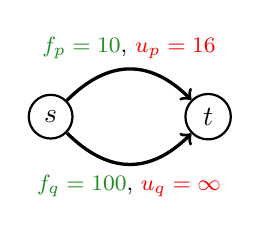
\begin{tikzpicture}[node distance={20mm}, thick, main/.style = {draw, circle}]
            \node[main] (s) {$s$}; 
            \node[main] (t) [right of=s] {$t$};
            \draw[->, very thick] (s) to [out=45, in=135, looseness=1.2] node[midway, above] {\footnotesize {\color{ForestGreen}$f_p = 10$}, {\color{Red} $u_p = 16$}} (t); 
            \draw[->, very thick] (s) to [out=-45, in=-135, looseness=1.2] node[midway, below] {\footnotesize {\color{ForestGreen}$f_q = 100$}, {\color{Red} $u_q = \infty$}} (t); 
        \end{tikzpicture} 
    
        {\color{red} $\text{Cost}_2 = 110$}
    \end{multicols}
    \caption{Comparison of resulting optimal network using each predicted demand. In bold are the arcs that are built to fulfill the respective demand. The cost of each network is different, despite identical prediction loss.}
    \label{fig:intro:example-optimization}
\end{figure}
\newpage

\section{Objectives and Contributions}

This project addresses the mismatch between the prediction and the optimization steps of a ND problem in which the commodity demands are uncertain. We integrate information about the optimization problem into the prediction step to obtain predicted demands that result in a cheaper downstream network. We refer to this process as \textit{Decision-Focused Learning (DFL)} or also \textit{Integrated Learning and Optimization (ILO)}. We have identified a gap in the DFL research. Most works focus on DFL for optimization problems with continuous variables and uncertainty in the objective function. Our project applies DFL to predicting demand in ND problems, which are combinatorial and present uncertainty in the constraints. Our objective is an exploratory study of DFL for ND. We aim to test existing approaches to identify their suitability for this problem.

In this project, we formulate an ND problem as a Contextual Stochastic Optimization (CSO) model. We study how to optimize such a model using a Prediction-Optimization pipeline, where the prediction step makes point predictions for the parameters and the optimization step solves the deterministic formulation of the ND problem. We show how to evaluate the performance of such a pipeline not in terms of prediction accuracy, but in terms of the cost of the downstream decisions. We show how the standard ways of evaluating the downstream optimization cost, regret-based losses, are mathematically ill-defined in cases where the uncertainty is in the constraints. 

We then formulate \textit{IO-Constraint}, a method that uses Inverse Optimization (IO) to train a linear prediction model that predicts demand from contextual information. We apply \textit{IO-Constraint} to synthetic instances of ND problems and compare the resulting network cost of \textit{IO-Constraint} to a linear regression model. We show that \textit{IO-Constraint} actually corresponds to Ordinary Linear Regression. Next, we observe that DFL may be viewed as appropriately weighting training examples in the loss function. We explore how changing the weighting of training examples that have a high impact on downstream costs in the loss function can improve the performance of the Prediction-Optimization pipeline. We present W-DFL, a nonlinear, multi-level optimization problem that defines the weightings that minimize the regret over the training dataset, and sketch ideas for finding effective weights using an iterative weight update algorithm.

\section{Thesis Structure}

This thesis is organized as follows. In Chapter~\ref{sec:litrev}, we review the existing research on ND, DFL, and IO. Using a common notation, we also introduce the mathematical notions from the literature used in our project. In Chapter~\ref{sec:methodology}, we formulate the ND problem and the Prediction-Optimization pipeline. We highlight issues related to evaluating the performance of a pipeline and the issues related to regret-based losses. We also formulate the \textit{IO-Constraint} method for training prediction losses and explore how reweighting training examples in the loss function when training a prediction model can improve downstream costs. In Chapter~\ref{sec:evaluation}, we evaluate the performance of \textit{IO-Constraint} on synthetic ND examples that should demonstrate the advantage of DFL methods. We show an example of how reweighting training examples improves the performance of a Prediction-Optimization pipeline on an ND problem and evaluate the iterative weight update method on that example. Chapter~\ref{sec:conclusion}, provides an overview of the work done in this thesis and presents avenues for future research.
